\documentclass[cal1spr16Lectures.tex]{subfiles}
%\AtBeginSubsection{
%	\begin{frame}[allowframebreaks]{}
%	\begin{multicols}{2}
%	\tableofcontents[currentsubsection]
%	\end{multicols}
%	\end{frame}
%	}
	
\begin{document}

%\section[Week 3]{Week 3: 1-5 February}

% % %
\subsubsection{\bf Monday 1 February}
\begin{frame}[allowframebreaks]{Mon 1 Feb}
\begin{itemize}%\footnotesize
\item GET YOUR CLICKER NOW.  	
\item EXAM 1 is one week from Friday.  Covers up to \S 3.1 (see the semester schedule of material on the course webpage).  \alert{You must attend your own lecture on exam day.}
\end{itemize}
\end{frame}

% % %
\begin{frame}
\begin{exe}
What are the vertical and horizontal asymptotes of $f(x)=\frac{x^2}{2x+1}$?
\end{exe}
\end{frame}

% % %
\subsubsection{Book Problems}
\begin{frame}
\begin{block}{2.5 Book Problems} 9-14, 15-33 (odds), 41-49 (odds), 53-59 (odds), 67  \end{block} 
\end{frame}

% % %
\subsection[2.6 Continuity]{\S 2.6 Continuity}
% % %

% % %
\begin{frame}{\S 2.6 Continuity}\footnotesize
Informally, a function $f$ is ``continuous at $x=a$" means for $x$-values anywhere close enough to $a$ the graph can be drawn without lifting a pencil.  In other words, no holes, breaks, asymptotes, etc.
\begin{dfn} A function $f$ is {\bf continuous} at $a$ means
\[\lim_{x \to a} f(x)=f(a).\]  
If $f$ is not continuous at $a$, then $a$ is a {\bf point of discontinuity}. \end{dfn}
\end{frame}

% % %
\subsubsection{Continuity Checklist}
% % %

% % %
\begin{frame}{\small Continuity Checklist}\footnotesize
In order to claim something is continuous, you must verify all three:
\begin{itemize}
\item[1.] \alert{$f(a)$ is defined} (i.e., $a$ is in the domain of $f$ -- no holes, asymptotes).
\item[2.] \alert{$\displaystyle\lim_{x \to a} f(x)$ exists.}  You must check both sides and make sure they equal the same number.
\item[3.] \alert{$\displaystyle\lim_{x \to a} f(x) = f(a)$} (i.e., the value of $f$ equals the limit of $f$ at $a$).  
\begin{que} What is an example of a function that satisfies this condition? \end{que}
\end{itemize}
\end{frame}

% % %
\begin{frame}\footnotesize
\begin{columns}[T]
	\begin{column}{.65\textwidth}
		\begin{ex} \begin{itemize}
		\item Where are the points of discontinuity of the function below?  
		\item Which aspects of the checklist fail?
		\end{itemize}
		\centering{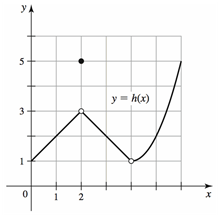
\includegraphics[scale=0.72]{pictures/Ch2Sect2_Exer7}}
		\end{ex}
	\end{column}
	\begin{column}{.4\textwidth}
	\vspace{8pc}
		recall (Continuity Checklist):
			\vspace{-1pc}
			\begin{itemize}
			\item[1.] function is defined
			\item[2.] the two-sided limit exists
			\item[3.] 2.\;=\;1.
			\end{itemize}
	\end{column}
\end{columns}
\end{frame}

% % %
\subsubsection{Continuity Rules}
% % %

% % %
\begin{frame}{\small Continuity Rules}
If $f$ and $g$ are continuous at $a$, then the following functions are also continuous at $a$.  Assume $c$ is a constant and $n>0$ is an integer.
\begin{itemize}
\item[1.] $f+g$
\item[2.] $f-g$
\item[3.] $cf$
\item[4.] $fg$
\item[5.] $\frac{f}{g}$, provided $g(a)\ne 0$
\item[6.] $[f(x)]^n$
\end{itemize}
\end{frame}

% % %
\begin{frame}
From the rules above, we can deduce:
\begin{itemize}
\item[1.] Polynomials are continuous for all $x=a$.
\item[2.] Rational functions are continuous at all $x=a$ except for the points where the denominator is zero.  
\item[3.] If $g$ is continuous at $a$ and $f$ is continuous at $g(a)$, then the composite function $f \circ g$ is continuous at $a$.
\end{itemize}
\end{frame}

% % %
\subsubsection{Continuity on an Interval}
% % %

% % %
\begin{frame}{\small Continuity on an Interval}\footnotesize 
Consider the cases where $f$ is not defined past a certain point. 
\begin{dfn}
A function $f$ is {\bf continuous from the left} (or {\bf left-continuous}) at $a$ means
\[\lim_{x \to a^-} f(x)=f(a);\]
a function $f$ is {\bf continuous from the right} (or {\bf right-continuous}) at $a$ means
\[\lim_{x \to a^+} f(x)=f(a).\]
\end{dfn}
\end{frame}

% % %
\begin{frame}
\begin{dfn} A function $f$ is {\bf continuous on an interval $I$} means it is continuous at all points of $I$. \end{dfn}  
Notation: Intervals are usually written 
\[\left[a,b\right],\;\left(a,b\right],\;\left[a,b\right),\text{ or }\left(a,b\right).\]
When $I$ contains its endpoints, ``continuity on $I$" means continuous from the right or left at the endpoints.
\end{frame}

\end{document}